\documentclass{article}\usepackage[]{graphicx}\usepackage[]{color}
%% maxwidth is the original width if it is less than linewidth
%% otherwise use linewidth (to make sure the graphics do not exceed the margin)
\makeatletter
\def\maxwidth{ %
  \ifdim\Gin@nat@width>\linewidth
    \linewidth
  \else
    \Gin@nat@width
  \fi
}
\makeatother

\definecolor{fgcolor}{rgb}{0.345, 0.345, 0.345}
\newcommand{\hlnum}[1]{\textcolor[rgb]{0.686,0.059,0.569}{#1}}%
\newcommand{\hlstr}[1]{\textcolor[rgb]{0.192,0.494,0.8}{#1}}%
\newcommand{\hlcom}[1]{\textcolor[rgb]{0.678,0.584,0.686}{\textit{#1}}}%
\newcommand{\hlopt}[1]{\textcolor[rgb]{0,0,0}{#1}}%
\newcommand{\hlstd}[1]{\textcolor[rgb]{0.345,0.345,0.345}{#1}}%
\newcommand{\hlkwa}[1]{\textcolor[rgb]{0.161,0.373,0.58}{\textbf{#1}}}%
\newcommand{\hlkwb}[1]{\textcolor[rgb]{0.69,0.353,0.396}{#1}}%
\newcommand{\hlkwc}[1]{\textcolor[rgb]{0.333,0.667,0.333}{#1}}%
\newcommand{\hlkwd}[1]{\textcolor[rgb]{0.737,0.353,0.396}{\textbf{#1}}}%
\let\hlipl\hlkwb

\usepackage{framed}
\makeatletter
\newenvironment{kframe}{%
 \def\at@end@of@kframe{}%
 \ifinner\ifhmode%
  \def\at@end@of@kframe{\end{minipage}}%
  \begin{minipage}{\columnwidth}%
 \fi\fi%
 \def\FrameCommand##1{\hskip\@totalleftmargin \hskip-\fboxsep
 \colorbox{shadecolor}{##1}\hskip-\fboxsep
     % There is no \\@totalrightmargin, so:
     \hskip-\linewidth \hskip-\@totalleftmargin \hskip\columnwidth}%
 \MakeFramed {\advance\hsize-\width
   \@totalleftmargin\z@ \linewidth\hsize
   \@setminipage}}%
 {\par\unskip\endMakeFramed%
 \at@end@of@kframe}
\makeatother

\definecolor{shadecolor}{rgb}{.97, .97, .97}
\definecolor{messagecolor}{rgb}{0, 0, 0}
\definecolor{warningcolor}{rgb}{1, 0, 1}
\definecolor{errorcolor}{rgb}{1, 0, 0}
\newenvironment{knitrout}{}{} % an empty environment to be redefined in TeX

\usepackage{alltt}

\usepackage{hyperref}

\title{Package \textbf{CompSign}}
\author{Lena Morrill}
\date{October 2017}
\IfFileExists{upquote.sty}{\usepackage{upquote}}{}
\begin{document}

\maketitle

\textbf{CompSign} is a package for yadayada... overlooked that mutational signatures are compositional in nature yadayada. The reference manual can be found \href{https://github.com/lm687/CompSign/blob/master/CompSign.pdf}{here}.

\tableofcontents

\begin{knitrout}
\definecolor{shadecolor}{rgb}{0.969, 0.969, 0.969}\color{fgcolor}\begin{kframe}
\begin{alltt}
\hlstd{knitr}\hlopt{::}\hlstd{opts_chunk}\hlopt{$}\hlkwd{set}\hlstd{(}\hlkwc{cache} \hlstd{=} \hlnum{FALSE}\hlstd{)}
\end{alltt}
\end{kframe}
\end{knitrout}

\begin{knitrout}
\definecolor{shadecolor}{rgb}{0.969, 0.969, 0.969}\color{fgcolor}\begin{kframe}
\begin{alltt}
\hlcom{## This chunk was last ran in}
\hlkwd{timestamp}\hlstd{()}
\end{alltt}
\begin{verbatim}
## ##------ Tue Nov 20 15:44:49 2018 ------##
\end{verbatim}
\begin{alltt}
\hlcom{## install latest version}
\hlkwd{library}\hlstd{(devtools)}
\hlcom{#devtools::install_github("lm687/CompSign")}
\hlkwd{library}\hlstd{(CompSign)}
\hlkwd{library}\hlstd{(compositions)}
\end{alltt}


{\ttfamily\noindent\itshape\color{messagecolor}{\#\# Loading required package: tensorA}}

{\ttfamily\noindent\itshape\color{messagecolor}{\#\# \\\#\# Attaching package: 'tensorA'}}

{\ttfamily\noindent\itshape\color{messagecolor}{\#\# The following object is masked from 'package:base':\\\#\# \\\#\#\ \ \ \  norm}}

{\ttfamily\noindent\itshape\color{messagecolor}{\#\# Loading required package: robustbase}}

{\ttfamily\noindent\itshape\color{messagecolor}{\#\# Loading required package: energy}}

{\ttfamily\noindent\itshape\color{messagecolor}{\#\# Loading required package: bayesm}}

{\ttfamily\noindent\itshape\color{messagecolor}{\#\# Welcome to compositions, a package for compositional data analysis.\\\#\# Find an intro with "{}? compositions"{}}}

{\ttfamily\noindent\itshape\color{messagecolor}{\#\# \\\#\# Attaching package: 'compositions'}}

{\ttfamily\noindent\itshape\color{messagecolor}{\#\# The following objects are masked from 'package:stats':\\\#\# \\\#\#\ \ \ \  cor, cov, dist, var}}

{\ttfamily\noindent\itshape\color{messagecolor}{\#\# The following objects are masked from 'package:base':\\\#\# \\\#\#\ \ \ \  \%*\%, scale, scale.default}}\end{kframe}
\end{knitrout}

\begin{knitrout}
\definecolor{shadecolor}{rgb}{0.969, 0.969, 0.969}\color{fgcolor}\begin{kframe}
\begin{alltt}
\hlcom{## if the folder data/ is not in github}
\hlkwa{for}\hlstd{(i} \hlkwa{in} \hlkwd{list.files}\hlstd{(}\hlstr{"../data/"}\hlstd{,} \hlkwc{pattern} \hlstd{=} \hlstr{"*rda"}\hlstd{,} \hlkwc{full.names} \hlstd{=} \hlnum{TRUE}\hlstd{))\{}\hlkwd{load}\hlstd{(i)\}}
\end{alltt}
\end{kframe}
\end{knitrout}

\begin{knitrout}
\definecolor{shadecolor}{rgb}{0.969, 0.969, 0.969}\color{fgcolor}\begin{kframe}
\begin{alltt}
\hlcom{## This chunk was last ran in}
\hlkwd{timestamp}\hlstd{()}
\end{alltt}
\begin{verbatim}
## ##------ Tue Nov 20 15:44:50 2018 ------##
\end{verbatim}
\begin{alltt}
\hlcom{##########################}
\hlcom{####### Dummy data #######}
\hlcom{##########################}

\hlcom{### Example of matrix transformed into sign object}
\hlstd{input_dummy} \hlkwb{<-} \hlkwd{matrix}\hlstd{(}\hlkwd{runif}\hlstd{(}\hlnum{100}\hlstd{),} \hlnum{4}\hlstd{)}
\hlkwd{colnames}\hlstd{(input_dummy)} \hlkwb{<-} \hlkwd{paste0}\hlstd{(}\hlstr{'s'}\hlstd{,} \hlnum{1}\hlopt{:}\hlnum{25}\hlstd{);} \hlkwd{rownames}\hlstd{(input_dummy)} \hlkwb{<-} \hlkwd{paste0}\hlstd{(}\hlstr{'sam'}\hlstd{,} \hlnum{1}\hlopt{:}\hlnum{4}\hlstd{)}
\hlstd{sign_dummy} \hlkwb{<-} \hlkwd{to_sign}\hlstd{(input_dummy)}
\end{alltt}
\end{kframe}
\end{knitrout}

\section{Summarise the signature matrix}
\begin{knitrout}
\definecolor{shadecolor}{rgb}{0.969, 0.969, 0.969}\color{fgcolor}\begin{kframe}
\begin{alltt}
\hlcom{## This chunk was last ran in}
\hlkwd{timestamp}\hlstd{()}
\end{alltt}
\begin{verbatim}
## ##------ Tue Nov 20 15:44:50 2018 ------##
\end{verbatim}
\begin{alltt}
\hlkwd{add_together_matrix}\hlstd{(sign_dummy)}
\end{alltt}
\begin{verbatim}
## An object of class "sign"
## Slot "id":
## [1] "input_dummy"
## 
## Slot "id_samples":
## [1] "sam1" "sam2" "sam3" "sam4"
## 
## Slot "id_signatures":
##  [1] "s1"  "s2"  "s3"  "s4"  "s5"  "s6"  "s7"  "s8"  "s9"  "s10" "s11"
## [12] "s12" "s13" "s14" "s15" "s16" "s17" "s18" "s19" "s20" "s21" "s22"
## [23] "s23" "s24" "s25"
## 
## Slot "count_matrix":
##             s1        s2         s3        s4        s5        s6
## sam1 0.7541314 0.4970128 0.78211567 0.3915332 0.2738219 0.2005642
## sam2 0.7812332 0.8232943 0.22102898 0.1358599 0.9786203 0.4597861
## sam3 0.4351710 0.4052233 0.61169752 0.2982947 0.9425812 0.9734695
## sam4 0.2483642 0.8148358 0.08488753 0.6137194 0.2942012 0.4174360
##             s7        s8        s9       s10       s11        s12
## sam1 0.7749699 0.9754341 0.7637598 0.6763901 0.0095364 0.52851290
## sam2 0.6510488 0.8995055 0.1498146 0.8108928 0.8500328 0.52726926
## sam3 0.0927079 0.4473260 0.7640837 0.3240883 0.1607237 0.04775178
## sam4 0.7322792 0.3212439 0.4094843 0.5324957 0.9396786 0.31369197
##            s13       s14       s15       s16        s17        s18
## sam1 0.1959873 0.2996425 0.2547190 0.3659506 0.80996888 0.18370775
## sam2 0.5323840 0.0236303 0.7940158 0.5731402 0.44363277 0.07648741
## sam3 0.8032507 0.5102668 0.1292824 0.3150606 0.76647091 0.47437104
## sam4 0.8661609 0.3289789 0.3239946 0.4355564 0.01661512 0.72830942
##            s19        s20       s21       s22       s23       s24
## sam1 0.8643979 0.20015968 0.7489268 0.6481179 0.6783852 0.4618235
## sam2 0.5533880 0.34117733 0.5923476 0.6612199 0.4517486 0.8622700
## sam3 0.6750658 0.29387013 0.3242528 0.7936309 0.7068090 0.8911294
## sam4 0.3262684 0.08579528 0.1805006 0.3249219 0.3352801 0.2316338
##             s25
## sam1 0.50067933
## sam2 0.02525199
## sam3 0.76196463
## sam4 0.36252690
## 
## Slot "modified":
## [1] TRUE
\end{verbatim}
\begin{alltt}
\hlstd{results_sumarise} \hlkwb{<-} \hlkwd{summarise}\hlstd{(}\hlkwd{add_together_matrix}\hlstd{(sign_dummy))}
\hlstd{results_sumarise}\hlopt{$}\hlstd{General}
\end{alltt}
\begin{verbatim}
## [1] "Object of class sign"
\end{verbatim}
\end{kframe}
\end{knitrout}

\section{Linear model for numerical predictors}
\begin{knitrout}
\definecolor{shadecolor}{rgb}{0.969, 0.969, 0.969}\color{fgcolor}\begin{kframe}
\begin{alltt}
\hlcom{## This chunk was last ran in}
\hlkwd{timestamp}\hlstd{()}
\end{alltt}
\begin{verbatim}
## ##------ Tue Nov 20 15:44:50 2018 ------##
\end{verbatim}
\begin{alltt}
\hlstd{tmp_merged_compositional} \hlkwb{<-} \hlkwd{new}\hlstd{(}\hlstr{"merged_compositional"}\hlstd{,}
                                \hlkwc{id}\hlstd{=}\hlstr{'adas'}\hlstd{,}
                                \hlkwc{id_samples}\hlstd{=}\hlkwd{paste0}\hlstd{(}\hlstr{"sam"}\hlstd{,} \hlnum{1}\hlopt{:}\hlnum{30}\hlstd{),}
                                \hlkwc{id_signatures}\hlstd{=} \hlkwd{c}\hlstd{(}\hlstr{'s1'}\hlstd{,} \hlstr{'s2'}\hlstd{,} \hlstr{'s3'}\hlstd{,} \hlstr{'s4'}\hlstd{),} \hlcom{## signature names}
                                \hlkwc{count_matrix}\hlstd{=MCMCpack}\hlopt{::}\hlkwd{rdirichlet}\hlstd{(}\hlnum{30}\hlstd{,} \hlkwd{c}\hlstd{(}\hlnum{1}\hlstd{,}\hlnum{1}\hlstd{,}\hlnum{1}\hlstd{,}\hlnum{1}\hlstd{)),}
                                \hlkwc{df}\hlstd{=}\hlkwd{data.frame}\hlstd{(}\hlkwc{a}\hlstd{=}\hlkwd{sample}\hlstd{(}\hlnum{1}\hlopt{:}\hlnum{1e4}\hlstd{,} \hlnum{30}\hlstd{),} \hlkwc{b}\hlstd{=}\hlkwd{rep}\hlstd{(}\hlnum{10}\hlstd{,} \hlnum{30}\hlstd{)))}
\hlkwd{comp_lm}\hlstd{(tmp_merged_compositional)}
\end{alltt}
\begin{verbatim}
## [[1]]
## Response Y1 :
## 
## Call:
## lm(formula = Y1 ~ as.matrix((x@df)[, indices_predictor]))
## 
## Residuals:
##     Min      1Q  Median      3Q     Max 
## -3.2627 -1.0761  0.1978  0.8880  2.3941 
## 
## Coefficients: (1 not defined because of singularities)
##                                           Estimate Std. Error t value
## (Intercept)                             -7.041e-01  5.485e-01  -1.284
## as.matrix((x@df)[, indices_predictor])a  8.013e-05  9.474e-05   0.846
## as.matrix((x@df)[, indices_predictor])b         NA         NA      NA
##                                         Pr(>|t|)
## (Intercept)                                0.210
## as.matrix((x@df)[, indices_predictor])a    0.405
## as.matrix((x@df)[, indices_predictor])b       NA
## 
## Residual standard error: 1.462 on 28 degrees of freedom
## Multiple R-squared:  0.02491,	Adjusted R-squared:  -0.009916 
## F-statistic: 0.7153 on 1 and 28 DF,  p-value: 0.4049
## 
## 
## Response Y2 :
## 
## Call:
## lm(formula = Y2 ~ as.matrix((x@df)[, indices_predictor]))
## 
## Residuals:
##     Min      1Q  Median      3Q     Max 
## -2.2764 -0.6695 -0.0375  1.0616  1.6511 
## 
## Coefficients: (1 not defined because of singularities)
##                                           Estimate Std. Error t value
## (Intercept)                             -4.633e-01  4.304e-01  -1.076
## as.matrix((x@df)[, indices_predictor])a  8.057e-05  7.434e-05   1.084
## as.matrix((x@df)[, indices_predictor])b         NA         NA      NA
##                                         Pr(>|t|)
## (Intercept)                                0.291
## as.matrix((x@df)[, indices_predictor])a    0.288
## as.matrix((x@df)[, indices_predictor])b       NA
## 
## Residual standard error: 1.147 on 28 degrees of freedom
## Multiple R-squared:  0.04026,	Adjusted R-squared:  0.005979 
## F-statistic: 1.174 on 1 and 28 DF,  p-value: 0.2877
## 
## 
## Response Y3 :
## 
## Call:
## lm(formula = Y3 ~ as.matrix((x@df)[, indices_predictor]))
## 
## Residuals:
##     Min      1Q  Median      3Q     Max 
## -6.5523 -0.7553  0.2355  1.1816  2.9865 
## 
## Coefficients: (1 not defined because of singularities)
##                                           Estimate Std. Error t value
## (Intercept)                             -0.6268989  0.7638802  -0.821
## as.matrix((x@df)[, indices_predictor])a  0.0001010  0.0001319   0.766
## as.matrix((x@df)[, indices_predictor])b         NA         NA      NA
##                                         Pr(>|t|)
## (Intercept)                                0.419
## as.matrix((x@df)[, indices_predictor])a    0.450
## as.matrix((x@df)[, indices_predictor])b       NA
## 
## Residual standard error: 2.036 on 28 degrees of freedom
## Multiple R-squared:  0.02051,	Adjusted R-squared:  -0.01448 
## F-statistic: 0.5862 on 1 and 28 DF,  p-value: 0.4503
\end{verbatim}
\end{kframe}
\end{knitrout}

\section{Importing data}
\begin{knitrout}
\definecolor{shadecolor}{rgb}{0.969, 0.969, 0.969}\color{fgcolor}\begin{kframe}
\begin{alltt}
\hlcom{## This chunk was last ran in}
\hlkwd{timestamp}\hlstd{()}
\end{alltt}
\begin{verbatim}
## ##------ Tue Nov 20 15:44:51 2018 ------##
\end{verbatim}
\begin{alltt}
\hlkwd{biplot}\hlstd{(}\hlkwd{princomp}\hlstd{(}\hlkwd{acomp}\hlstd{(MCMCpack}\hlopt{::}\hlkwd{rdirichlet}\hlstd{(}\hlnum{30}\hlstd{,} \hlkwd{rep}\hlstd{(}\hlnum{1}\hlstd{,} \hlnum{4}\hlstd{)))))}
\end{alltt}
\end{kframe}
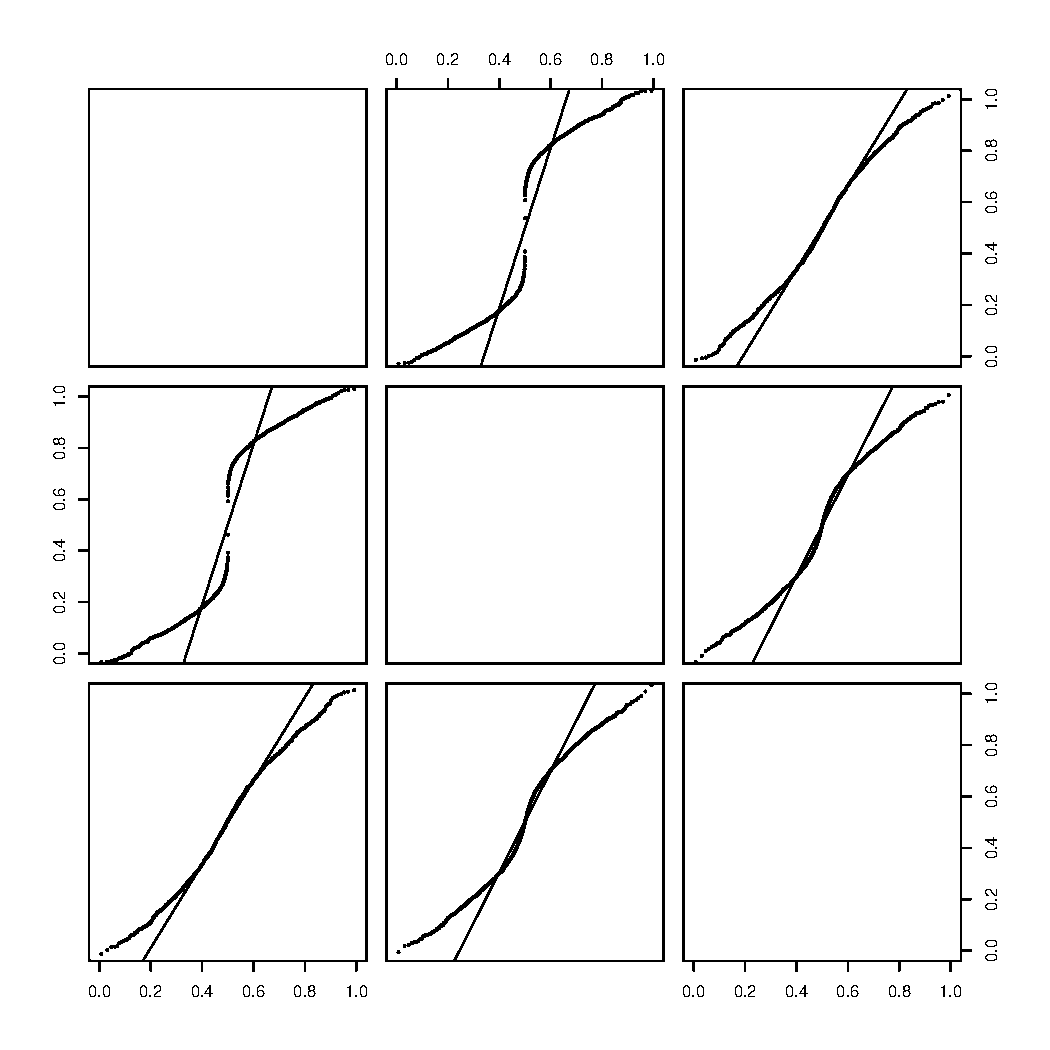
\includegraphics[width=\maxwidth]{figure/unnamed-chunk-7-1} 

\end{knitrout}

\section{Other}
\begin{enumerate}
\item Test for normality as follows:
\begin{knitrout}
\definecolor{shadecolor}{rgb}{0.969, 0.969, 0.969}\color{fgcolor}\begin{kframe}
\begin{alltt}
\hlcom{## This chunk was last ran in}
\hlkwd{timestamp}\hlstd{()}
\end{alltt}
\begin{verbatim}
## ##------ Tue Nov 20 15:44:52 2018 ------##
\end{verbatim}
\begin{alltt}
\hlkwd{data}\hlstd{(two_normal_pops)}
\hlkwd{par}\hlstd{(}\hlkwc{mfrow}\hlstd{=}\hlkwd{c}\hlstd{(}\hlnum{1}\hlstd{,}\hlnum{2}\hlstd{))}
\hlkwd{qqnorm.acomp}\hlstd{(}\hlkwd{acomp}\hlstd{(two_normal_pops}\hlopt{@}\hlkwc{count_matrix}\hlstd{),} \hlkwc{pch}\hlstd{=}\hlnum{19}\hlstd{,} \hlkwc{cex}\hlstd{=}\hlnum{0.2}\hlstd{)}
\end{alltt}
\end{kframe}
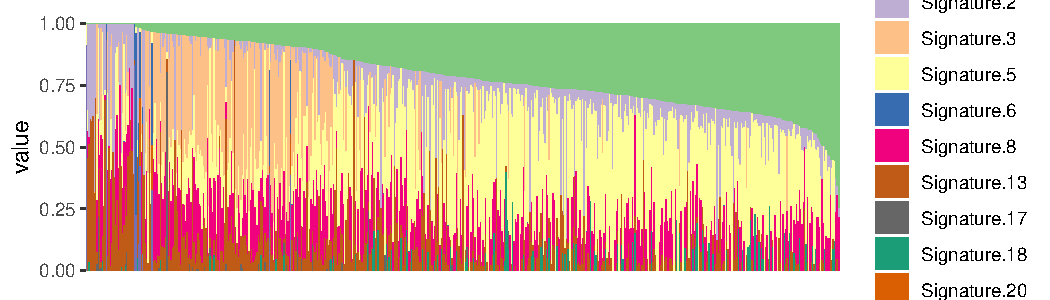
\includegraphics[width=\maxwidth]{figure/unnamed-chunk-8-1} 
\begin{kframe}\begin{alltt}
\hlkwd{qqnorm.acomp}\hlstd{(}\hlkwd{acomp}\hlstd{(two_normal_pops}\hlopt{@}\hlkwc{count_matrix}\hlstd{[}\hlnum{1}\hlopt{:}\hlnum{1000}\hlstd{,]),} \hlkwc{pch}\hlstd{=}\hlnum{19}\hlstd{,} \hlkwc{cex}\hlstd{=}\hlnum{0.2}\hlstd{,} \hlkwc{plot.it}\hlstd{=}\hlnum{FALSE}\hlstd{)}
\end{alltt}


{\ttfamily\noindent\color{warningcolor}{\#\# Warning in plot.window(...): "{}plot.it"{} is not a graphical parameter}}

{\ttfamily\noindent\color{warningcolor}{\#\# Warning in plot.xy(xy, type, ...): "{}plot.it"{} is not a graphical parameter}}

{\ttfamily\noindent\color{warningcolor}{\#\# Warning in title(...): "{}plot.it"{} is not a graphical parameter}}

{\ttfamily\noindent\color{warningcolor}{\#\# Warning in plot.window(...): "{}plot.it"{} is not a graphical parameter}}

{\ttfamily\noindent\color{warningcolor}{\#\# Warning in plot.xy(xy, type, ...): "{}plot.it"{} is not a graphical parameter}}

{\ttfamily\noindent\color{warningcolor}{\#\# Warning in title(...): "{}plot.it"{} is not a graphical parameter}}

{\ttfamily\noindent\color{warningcolor}{\#\# Warning in axis(side = side, at = at, labels = labels, ...): "{}plot.it"{} is not a graphical parameter}}

{\ttfamily\noindent\color{warningcolor}{\#\# Warning in plot.xy(xy.coords(x, y), type = type, ...): "{}plot.it"{} is not a graphical parameter}}

{\ttfamily\noindent\color{warningcolor}{\#\# Warning in plot.window(...): "{}plot.it"{} is not a graphical parameter}}

{\ttfamily\noindent\color{warningcolor}{\#\# Warning in plot.xy(xy, type, ...): "{}plot.it"{} is not a graphical parameter}}

{\ttfamily\noindent\color{warningcolor}{\#\# Warning in title(...): "{}plot.it"{} is not a graphical parameter}}

{\ttfamily\noindent\color{warningcolor}{\#\# Warning in axis(side = side, at = at, labels = labels, ...): "{}plot.it"{} is not a graphical parameter}}

{\ttfamily\noindent\color{warningcolor}{\#\# Warning in plot.xy(xy.coords(x, y), type = type, ...): "{}plot.it"{} is not a graphical parameter}}

{\ttfamily\noindent\color{warningcolor}{\#\# Warning in plot.window(...): "{}plot.it"{} is not a graphical parameter}}

{\ttfamily\noindent\color{warningcolor}{\#\# Warning in plot.xy(xy, type, ...): "{}plot.it"{} is not a graphical parameter}}

{\ttfamily\noindent\color{warningcolor}{\#\# Warning in title(...): "{}plot.it"{} is not a graphical parameter}}

{\ttfamily\noindent\color{warningcolor}{\#\# Warning in axis(side = side, at = at, labels = labels, ...): "{}plot.it"{} is not a graphical parameter}}

{\ttfamily\noindent\color{warningcolor}{\#\# Warning in plot.xy(xy.coords(x, y), type = type, ...): "{}plot.it"{} is not a graphical parameter}}

{\ttfamily\noindent\color{warningcolor}{\#\# Warning in plot.window(...): "{}plot.it"{} is not a graphical parameter}}

{\ttfamily\noindent\color{warningcolor}{\#\# Warning in plot.xy(xy, type, ...): "{}plot.it"{} is not a graphical parameter}}

{\ttfamily\noindent\color{warningcolor}{\#\# Warning in title(...): "{}plot.it"{} is not a graphical parameter}}

{\ttfamily\noindent\color{warningcolor}{\#\# Warning in plot.window(...): "{}plot.it"{} is not a graphical parameter}}

{\ttfamily\noindent\color{warningcolor}{\#\# Warning in plot.xy(xy, type, ...): "{}plot.it"{} is not a graphical parameter}}

{\ttfamily\noindent\color{warningcolor}{\#\# Warning in title(...): "{}plot.it"{} is not a graphical parameter}}

{\ttfamily\noindent\color{warningcolor}{\#\# Warning in plot.xy(xy.coords(x, y), type = type, ...): "{}plot.it"{} is not a graphical parameter}}

{\ttfamily\noindent\color{warningcolor}{\#\# Warning in plot.window(...): "{}plot.it"{} is not a graphical parameter}}

{\ttfamily\noindent\color{warningcolor}{\#\# Warning in plot.xy(xy, type, ...): "{}plot.it"{} is not a graphical parameter}}

{\ttfamily\noindent\color{warningcolor}{\#\# Warning in title(...): "{}plot.it"{} is not a graphical parameter}}

{\ttfamily\noindent\color{warningcolor}{\#\# Warning in axis(side = side, at = at, labels = labels, ...): "{}plot.it"{} is not a graphical parameter}}

{\ttfamily\noindent\color{warningcolor}{\#\# Warning in plot.xy(xy.coords(x, y), type = type, ...): "{}plot.it"{} is not a graphical parameter}}

{\ttfamily\noindent\color{warningcolor}{\#\# Warning in plot.window(...): "{}plot.it"{} is not a graphical parameter}}

{\ttfamily\noindent\color{warningcolor}{\#\# Warning in plot.xy(xy, type, ...): "{}plot.it"{} is not a graphical parameter}}

{\ttfamily\noindent\color{warningcolor}{\#\# Warning in title(...): "{}plot.it"{} is not a graphical parameter}}

{\ttfamily\noindent\color{warningcolor}{\#\# Warning in plot.xy(xy.coords(x, y), type = type, ...): "{}plot.it"{} is not a graphical parameter}}

{\ttfamily\noindent\color{warningcolor}{\#\# Warning in plot.window(...): "{}plot.it"{} is not a graphical parameter}}

{\ttfamily\noindent\color{warningcolor}{\#\# Warning in plot.xy(xy, type, ...): "{}plot.it"{} is not a graphical parameter}}

{\ttfamily\noindent\color{warningcolor}{\#\# Warning in title(...): "{}plot.it"{} is not a graphical parameter}}

{\ttfamily\noindent\color{warningcolor}{\#\# Warning in axis(side = side, at = at, labels = labels, ...): "{}plot.it"{} is not a graphical parameter}}

{\ttfamily\noindent\color{warningcolor}{\#\# Warning in axis(side = side, at = at, labels = labels, ...): "{}plot.it"{} is not a graphical parameter}}\end{kframe}
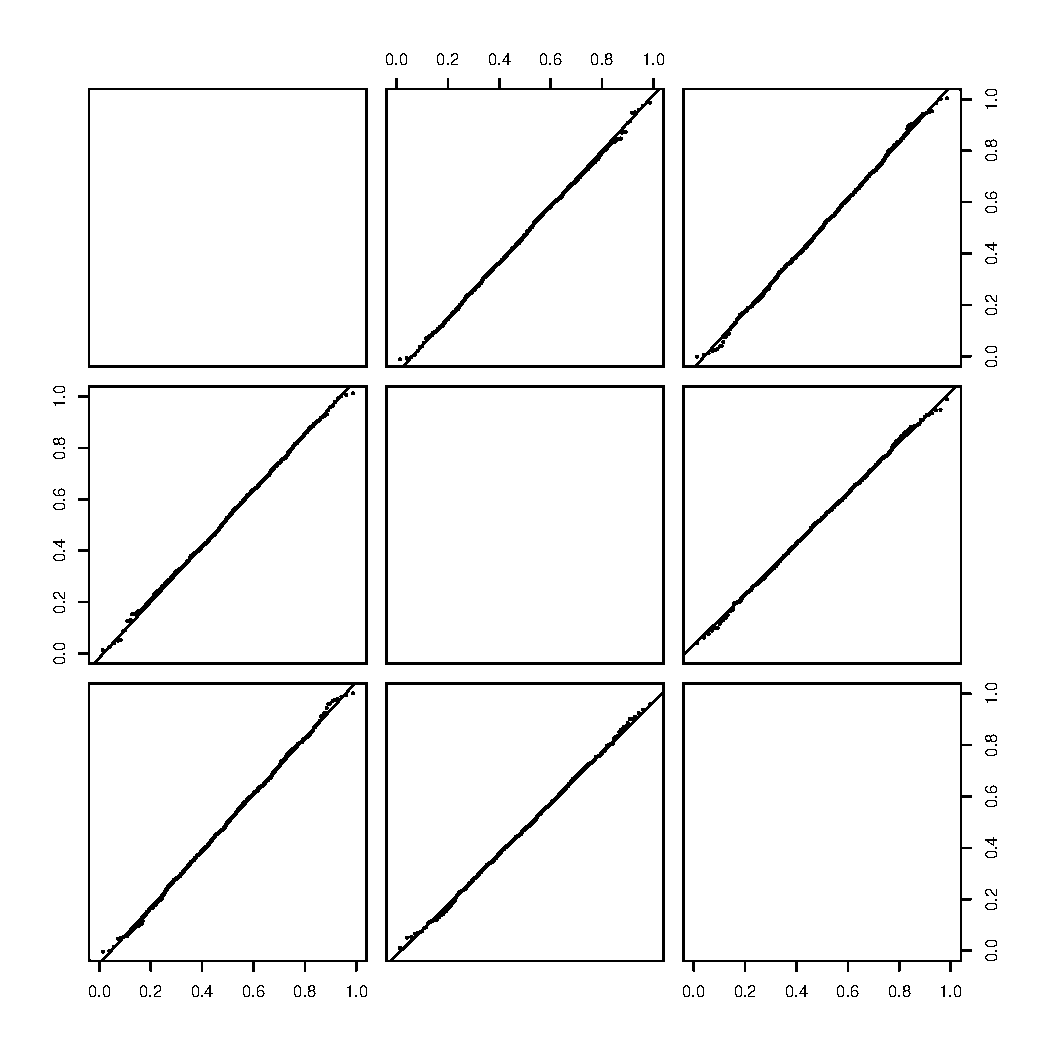
\includegraphics[width=\maxwidth]{figure/unnamed-chunk-8-2} 

\end{knitrout}
\end{enumerate}

\section{Clustering of samples}



\clearpage

\subsection{Testing hypotheses about two populations}
We might have our samples split into two categories; e.g. sex. As in Aithison 1986\cite{}, I follow a hierarchy of alternative hypotheses, from least to most complex.

Our first question is whether two populations have the same covariance and structure and center (i.e. if there is any distributional difference)

\begin{knitrout}
\definecolor{shadecolor}{rgb}{0.969, 0.969, 0.969}\color{fgcolor}\begin{kframe}
\begin{alltt}
\hlcom{## This chunk was last ran in}
\hlkwd{timestamp}\hlstd{()}
\end{alltt}
\begin{verbatim}
## ##------ Tue Nov 20 15:44:52 2018 ------##
\end{verbatim}
\begin{alltt}
\hlcom{##TODO!!}
\end{alltt}
\end{kframe}
\end{knitrout}

The next is whether the populations have a different center:

\begin{knitrout}
\definecolor{shadecolor}{rgb}{0.969, 0.969, 0.969}\color{fgcolor}\begin{kframe}
\begin{alltt}
\hlcom{## This chunk was last ran in}
\hlkwd{timestamp}\hlstd{()}
\end{alltt}
\begin{verbatim}
## ##------ Tue Nov 20 15:44:52 2018 ------##
\end{verbatim}
\begin{alltt}
\hlcom{## This dataset includes the two components above, as well as four others}
\hlcom{## (a total of seven)}
\hlkwd{data}\hlstd{(}\hlstr{"two_normal_pops_extended"}\hlstd{)}

\hlcom{## Data from the Landscape... paper}
\hlkwd{data}\hlstd{(}\hlstr{"Breast560"}\hlstd{)}

\hlstd{wrapper_compare_populations} \hlkwb{<-} \hlkwa{function}\hlstd{(}\hlkwc{predictors}\hlstd{,} \hlkwc{response}\hlstd{,} \hlkwc{...}\hlstd{)\{}
  \hlkwa{if}\hlstd{(}\hlkwd{length}\hlstd{(}\hlkwd{unique}\hlstd{(response))} \hlopt{==} \hlnum{2}\hlstd{)\{}
    \hlstd{tmp} \hlkwb{<-} \hlkwd{compare_populations}\hlstd{(predictors, response, ...)}
    \hlstd{tmp} \hlkwb{<-} \hlstd{tmp}\hlopt{$}\hlstd{info[}\hlnum{1}\hlopt{:}\hlnum{2}\hlstd{]}
    \hlstd{tmp}
  \hlstd{\}}
\hlstd{\}}

\hlstd{x} \hlkwb{<-} \hlkwd{do.call}\hlstd{(}\hlstr{'rbind'}\hlstd{,} \hlkwd{lapply}\hlstd{(}\hlnum{1}\hlopt{:}\hlkwd{ncol}\hlstd{(}\hlkwd{metadata}\hlstd{(Breast560)),}
       \hlkwa{function}\hlstd{(}\hlkwc{k}\hlstd{)\{}
         \hlkwd{wrapper_compare_populations}\hlstd{(}\hlkwc{predictors} \hlstd{=} \hlkwd{count_matrix}\hlstd{(Breast560),}
                                     \hlkwc{response} \hlstd{=} \hlkwd{metadata}\hlstd{(Breast560)[,k])}
         \hlstd{\}}
       \hlstd{))}
\end{alltt}


{\ttfamily\noindent\itshape\color{messagecolor}{\#\# Loading required package: Compositional}}

{\ttfamily\noindent\itshape\color{messagecolor}{\#\# \\\#\# Attaching package: 'Compositional'}}

{\ttfamily\noindent\itshape\color{messagecolor}{\#\# The following object is masked from 'package:compositions':\\\#\# \\\#\#\ \ \ \  alr}}\begin{alltt}
\hlstd{x}
\end{alltt}
\begin{verbatim}
##           test      p-value
## [1,] 215.35615 1.224333e-24
## [2,] 161.50152 3.522373e-18
## [3,] 235.90667 5.324172e-43
## [4,]  77.27718 1.042179e-11
\end{verbatim}
\end{kframe}
\end{knitrout}

\section{Datasets}
\subsection{Data for 560 breast cancer patients}
Data from 560 breast cancer patients is available as part of the document as well:

\begin{knitrout}
\definecolor{shadecolor}{rgb}{0.969, 0.969, 0.969}\color{fgcolor}\begin{kframe}
\begin{alltt}
\hlkwd{data}\hlstd{(}\hlstr{"Breast560"}\hlstd{)}
\hlkwd{metadata}\hlstd{(Breast560)[}\hlnum{1}\hlopt{:}\hlnum{4}\hlstd{,}\hlnum{1}\hlopt{:}\hlnum{5}\hlstd{]}
\end{alltt}
\begin{verbatim}
##         donor_gender donor_age_at_diagnosis donor_age_at_last_follow.up
## PD10010       female                     56            no_data_supplied
## PD10011       female                     75            no_data_supplied
## PD10014       female                     64            no_data_supplied
## PD11326       female                     38                          47
##          specimen_type donor_vital_status
## PD10010 tumour_primary              alive
## PD10011 tumour_primary              alive
## PD10014 tumour_primary           deceased
## PD11326 tumour_primary              alive
\end{verbatim}
\begin{alltt}
\hlkwd{count_matrix}\hlstd{(Breast560)[}\hlnum{1}\hlopt{:}\hlnum{4}\hlstd{,}\hlnum{1}\hlopt{:}\hlnum{5}\hlstd{]}
\end{alltt}
\begin{verbatim}
##         Signature.1 Signature.2 Signature.3 Signature.5 Signature.6
## PD10010  0.22386831  0.04197531   0.2181070   0.3374486           0
## PD10011  0.09840426  0.00000000   0.1791586   0.4514023           0
## PD10014  0.03290722  0.00000000   0.2859381   0.2812371           0
## PD11326  0.04040299  0.02596593   0.3579144   0.1606772           0
\end{verbatim}
\end{kframe}
\end{knitrout}

Not sure if this is correct
\begin{knitrout}
\definecolor{shadecolor}{rgb}{0.969, 0.969, 0.969}\color{fgcolor}\begin{kframe}
\begin{alltt}
\hlkwd{source}\hlstd{(}\hlstr{"../../CDA_in_Cancer/code/functions/basic_functions.R"}\hlstd{)}
\hlkwd{plotPCA}\hlstd{(}\hlkwd{ilr}\hlstd{(}\hlkwd{count_matrix}\hlstd{(Breast560)),} \hlkwc{pch}\hlstd{=}\hlnum{4}\hlstd{,} \hlkwc{col}\hlstd{=}\hlstr{'blue'}\hlstd{)}
\end{alltt}


{\ttfamily\noindent\itshape\color{messagecolor}{\#\# Loading required package: ggplot2}}\end{kframe}
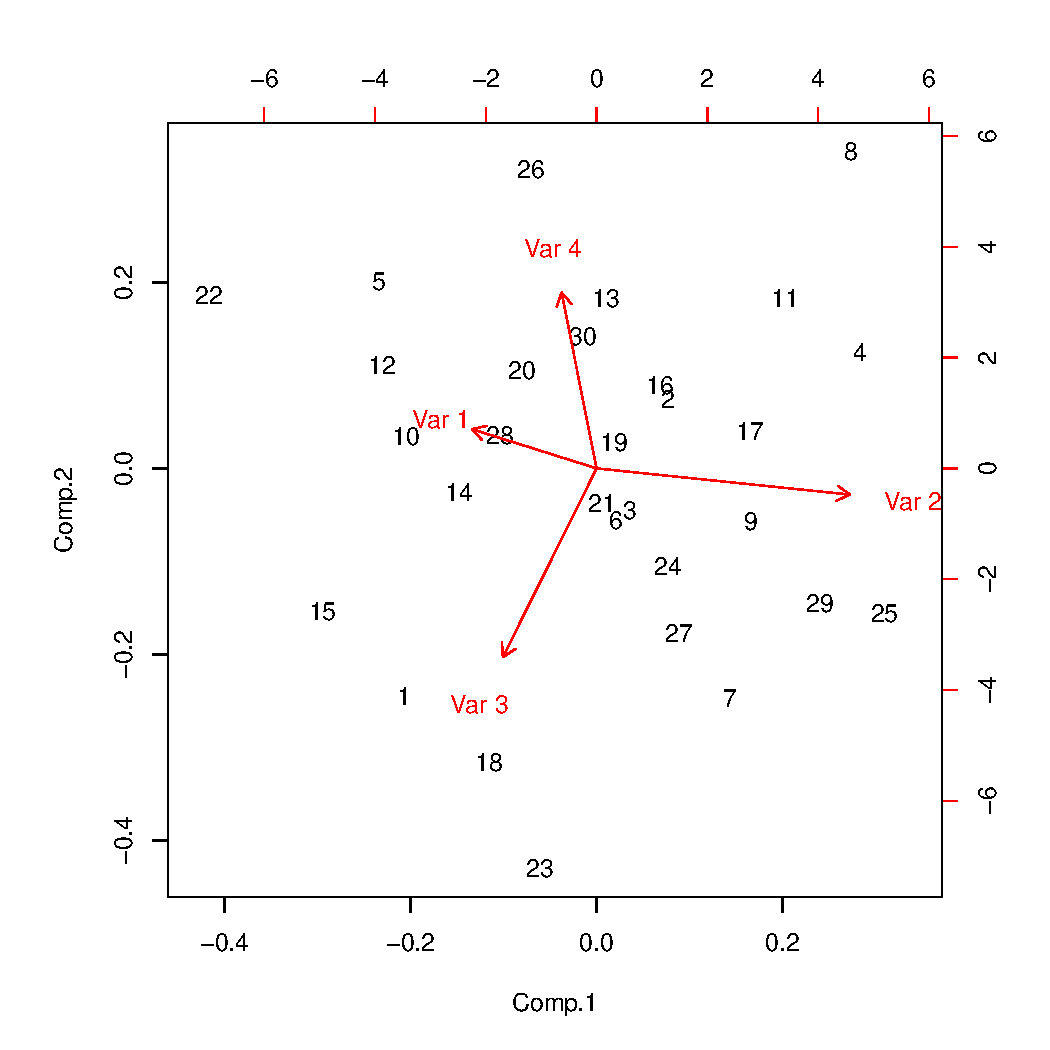
\includegraphics[width=\maxwidth]{figure/unnamed-chunk-13-1} 

\end{knitrout}


\subsection{Data for 12k TCGA samples, with ovarian cancer-derived CNA signatures}

\begin{knitrout}
\definecolor{shadecolor}{rgb}{0.969, 0.969, 0.969}\color{fgcolor}\begin{kframe}
\begin{alltt}
\hlkwd{timestamp}\hlstd{()}
\end{alltt}
\begin{verbatim}
## ##------ Tue Nov 20 15:44:53 2018 ------##
\end{verbatim}
\begin{alltt}
\hlkwd{data}\hlstd{(}\hlstr{"CNA_12K_TCGA"}\hlstd{)}

\hlkwd{dim}\hlstd{(}\hlkwd{metadata}\hlstd{(CNA_12K_TCGA))}
\end{alltt}
\begin{verbatim}
## [1] 10899    37
\end{verbatim}
\begin{alltt}
\hlkwd{dim}\hlstd{(}\hlkwd{count_matrix}\hlstd{(CNA_12K_TCGA))}
\end{alltt}
\begin{verbatim}
## [1] 10899     7
\end{verbatim}
\end{kframe}
\end{knitrout}

\section{Battery of tests}
\subsection{(ongoing) test for equality}

\begin{knitrout}
\definecolor{shadecolor}{rgb}{0.969, 0.969, 0.969}\color{fgcolor}\begin{kframe}
\begin{alltt}
\hlkwd{comp.test}\hlstd{(}\hlkwc{x} \hlstd{=} \hlkwd{count_matrix}\hlstd{(Breast560),}
                              \hlkwc{ina} \hlstd{=} \hlkwd{as.numeric}\hlstd{(}\hlkwd{as.factor}\hlstd{(}\hlkwd{metadata}\hlstd{(Breast560)}\hlopt{$}\hlstd{final.ER)),}
                              \hlkwc{test} \hlstd{=} \hlstr{"james"}\hlstd{,} \hlkwc{R} \hlstd{=} \hlnum{0}\hlstd{)}
\end{alltt}
\begin{verbatim}
## $note
## [1] "James test"
## 
## $mesoi
##                 X1        X2         X3       X4         X5        X6
## Sample 1 0.4947103 -1.717388 -0.8957869 1.702096 -0.1707924 0.1713026
## Sample 2 1.2111720  1.423396 -2.3153991 2.010485  0.3004208 0.6587258
##                X7       X8       X9       X10      X11
## Sample 1 1.442203 1.255236 1.216817 0.9930453 1.012318
## Sample 2 1.535435 1.119812 1.252353 1.0633045 1.044466
## 
## $info
##               test            p-value         correction 
##       2.790161e+02       9.100067e-51       1.046438e+00 
## corrected.critical 
##       2.058881e+01
\end{verbatim}
\end{kframe}
\end{knitrout}


\subsection{Logistic regression}
Based on ACDWR pg 200

\begin{knitrout}
\definecolor{shadecolor}{rgb}{0.969, 0.969, 0.969}\color{fgcolor}\begin{kframe}
\begin{alltt}
\hlcom{#setwd("~/Documents/PhD/CompSign/vignette_knitr/")}
\hlkwd{load}\hlstd{(}\hlstr{"../data/two_normal_pops_extended.rda"}\hlstd{)}
\hlkwd{load}\hlstd{(}\hlstr{"../data/two_normal_pops_extended.rda"}\hlstd{)}
\hlkwd{load}\hlstd{(}\hlstr{"../data/CNA_12K_TCGA.rda"}\hlstd{)}

\hlcom{## avoid perfect separation}
\hlstd{L} \hlkwb{<-} \hlkwd{length}\hlstd{((}\hlkwd{as.numeric}\hlstd{(}\hlkwd{metadata}\hlstd{(two_normal_pops_extended)[,}\hlnum{1}\hlstd{])))}
\hlstd{scramble} \hlkwb{<-} \hlkwd{sample}\hlstd{(}\hlnum{1}\hlopt{:}\hlstd{L,} \hlkwd{floor}\hlstd{(L}\hlopt{*}\hlnum{0.05}\hlstd{),} \hlkwc{replace} \hlstd{=} \hlnum{FALSE}\hlstd{)}

\hlstd{scrambled_labels} \hlkwb{<-} \hlstd{(}\hlkwd{as.numeric}\hlstd{(}\hlkwd{metadata}\hlstd{(two_normal_pops_extended)[,}\hlnum{1}\hlstd{]))}
\hlstd{scrambled_labels[scramble]} \hlkwb{<-} \hlnum{1}\hlopt{-}\hlstd{scrambled_labels[scramble]}

\hlstd{auxcomp} \hlkwb{<-} \hlkwd{scale}\hlstd{(}\hlkwd{ilr}\hlstd{(}\hlkwd{count_matrix}\hlstd{(two_normal_pops_extended)),}
                 \hlkwc{center} \hlstd{=} \hlnum{TRUE}\hlstd{,} \hlkwc{scale} \hlstd{=} \hlnum{FALSE}\hlstd{)}

\hlkwd{summary}\hlstd{(}\hlkwd{glm}\hlstd{(}\hlkwc{formula} \hlstd{= scrambled_labels} \hlopt{~} \hlkwd{ilr}\hlstd{(}\hlkwd{acomp}\hlstd{(}\hlkwd{count_matrix}\hlstd{(two_normal_pops_extended))),}
            \hlkwc{family} \hlstd{=} \hlkwd{binomial}\hlstd{(}\hlkwc{link} \hlstd{=} \hlstr{"logit"}\hlstd{)))}
\end{alltt}
\begin{verbatim}
## 
## Call:
## glm(formula = scrambled_labels ~ ilr(acomp(count_matrix(two_normal_pops_extended))), 
##     family = binomial(link = "logit"))
## 
## Deviance Residuals: 
##     Min       1Q   Median       3Q      Max  
## -2.8751  -0.2893  -0.1112   0.3276   3.0405  
## 
## Coefficients:
##                                                     Estimate Std. Error
## (Intercept)                                          0.20991    0.29938
## ilr(acomp(count_matrix(two_normal_pops_extended)))1  2.14865    0.08109
## ilr(acomp(count_matrix(two_normal_pops_extended)))2 -0.28219    0.20526
## ilr(acomp(count_matrix(two_normal_pops_extended)))3 -0.35257    0.13672
## ilr(acomp(count_matrix(two_normal_pops_extended)))4 -0.10861    0.11951
## ilr(acomp(count_matrix(two_normal_pops_extended)))5 -0.26914    0.11033
## ilr(acomp(count_matrix(two_normal_pops_extended)))6 -0.13039    0.10264
## ilr(acomp(count_matrix(two_normal_pops_extended)))7 -0.23026    0.10039
##                                                     z value Pr(>|z|)    
## (Intercept)                                           0.701  0.48322    
## ilr(acomp(count_matrix(two_normal_pops_extended)))1  26.499  < 2e-16 ***
## ilr(acomp(count_matrix(two_normal_pops_extended)))2  -1.375  0.16919    
## ilr(acomp(count_matrix(two_normal_pops_extended)))3  -2.579  0.00991 ** 
## ilr(acomp(count_matrix(two_normal_pops_extended)))4  -0.909  0.36346    
## ilr(acomp(count_matrix(two_normal_pops_extended)))5  -2.439  0.01471 *  
## ilr(acomp(count_matrix(two_normal_pops_extended)))6  -1.270  0.20395    
## ilr(acomp(count_matrix(two_normal_pops_extended)))7  -2.294  0.02181 *  
## ---
## Signif. codes:  0 '***' 0.001 '**' 0.01 '*' 0.05 '.' 0.1 ' ' 1
## 
## (Dispersion parameter for binomial family taken to be 1)
## 
##     Null deviance: 2772.46  on 1999  degrees of freedom
## Residual deviance:  822.17  on 1992  degrees of freedom
## AIC: 838.17
## 
## Number of Fisher Scoring iterations: 6
\end{verbatim}
\begin{alltt}
\hlstd{res} \hlkwb{<-} \hlkwd{comp_logistic}\hlstd{(}\hlkwd{count_matrix}\hlstd{(two_normal_pops), scrambled_labels)}
\end{alltt}


{\ttfamily\noindent\itshape\color{messagecolor}{\#\# Loading required package: nnet}}\begin{verbatim}
## # weights:  5 (4 variable)
## initial  value 1386.294361 
## final  value 446.109216 
## converged
\end{verbatim}
\begin{alltt}
\hlstd{res}
\end{alltt}
\begin{verbatim}
## $coefTransformed
## (Intercept)          X1          X2          X3 
##   0.3018093  -7.0122987   8.0287960  -0.7146880 
## 
## $summary
## Call:
## multinom(formula = as.formula(frm), data = dat)
## 
## Coefficients:
##                 Values Std. Err.
## (Intercept)  0.3018093 0.1344851
## X1          -7.0122987 0.3980051
## X2           8.0287960 0.3891784
## X3          -0.7146880 0.4310429
## 
## Residual Deviance: 892.2184 
## AIC: 898.2184 
## 
## $res
## Call:
## multinom(formula = as.formula(frm), data = dat)
## 
## Coefficients:
## (Intercept)          X1          X2          X3 
##   0.3018093  -7.0122987   8.0287960  -0.7146880 
## 
## Residual Deviance: 892.2184 
## AIC: 898.2184 
## 
## [[4]]
##    FP_FN_table
##       0   1
##   0 954  54
##   1  47 945
\end{verbatim}
\begin{alltt}
\hlstd{resB} \hlkwb{<-} \hlkwd{comp_logistic}\hlstd{(}\hlkwd{count_matrix}\hlstd{(two_normal_pops_extended), scrambled_labels)}
\end{alltt}
\begin{verbatim}
## # weights:  10 (9 variable)
## initial  value 1386.294361 
## iter  10 value 447.368111
## final  value 447.368099 
## converged
\end{verbatim}
\begin{alltt}
\hlstd{resB}
\end{alltt}
\begin{verbatim}
## $coefTransformed
## (Intercept)          X1          X2          X3          X4          X5 
##   0.3799636 -14.5095136  16.1858973  -1.4864019  -0.2664309   0.8591635 
##          X6          X7          X8 
##  -0.4274325   0.5919991  -0.5673174 
## 
## $summary
## Call:
## multinom(formula = as.formula(frm), data = dat)
## 
## Coefficients:
##                  Values Std. Err.
## (Intercept)   0.3799636 0.1600125
## X1          -14.5095136 0.7570415
## X2           16.1858973 0.7528891
## X3           -1.4864019 0.8965775
## X4           -0.2664309 0.9044187
## X5            0.8591635 0.8829952
## X6           -0.4274325 0.8830860
## X7            0.5919991 0.9177035
## X8           -0.5673174 0.8781700
## 
## Residual Deviance: 894.7362 
## AIC: 908.7362 
## 
## $res
## Call:
## multinom(formula = as.formula(frm), data = dat)
## 
## Coefficients:
## (Intercept)          X1          X2          X3          X4          X5 
##   0.3799636 -14.5095136  16.1858973  -1.4864019  -0.2664309   0.8591635 
##          X6          X7          X8 
##  -0.4274325   0.5919991  -0.5673174 
## 
## Residual Deviance: 894.7362 
## AIC: 908.7362 
## 
## [[4]]
##    FP_FN_table
##       0   1
##   0 954  54
##   1  46 946
\end{verbatim}
\begin{alltt}
\hlstd{resCNA_gender} \hlkwb{<-} \hlkwd{comp_logistic}\hlstd{(}\hlkwd{count_matrix}\hlstd{(}\hlkwd{cleanObject}\hlstd{(CNA_12K_TCGA,} \hlstr{'gender'}\hlstd{)),}
                              \hlkwd{metadata}\hlstd{(}\hlkwd{cleanObject}\hlstd{(CNA_12K_TCGA,} \hlstr{'gender'}\hlstd{))[,}\hlstr{'gender'}\hlstd{])}
\end{alltt}
\begin{verbatim}
## # weights:  9 (8 variable)
## initial  value 7535.896147 
## iter  10 value 7477.896938
## final  value 7477.896342 
## converged
\end{verbatim}
\begin{alltt}
\hlstd{resCNA_gender}
\end{alltt}
\begin{verbatim}
## $coefTransformed
## (Intercept)          s1          s2          s3          s4          s5 
##  -0.2991671   0.2381913  -1.5952762  -0.7137485  -0.3424139   1.1287220 
##          s6          s7 
##   1.1463550  -0.1609969 
## 
## $summary
## Call:
## multinom(formula = as.formula(frm), data = dat)
## 
## Coefficients:
##                 Values  Std. Err.
## (Intercept) -0.2991671 0.04634220
## s1           0.2381913 0.07069156
## s2          -1.5952762 0.34187887
## s3          -0.7137485 0.15918132
## s4          -0.3424139 0.22213187
## s5           1.1287220 0.15577367
## s6           1.1463550 0.25201363
## s7          -0.1609969 0.19798834
## 
## Residual Deviance: 14955.79 
## AIC: 14969.79 
## 
## $res
## Call:
## multinom(formula = as.formula(frm), data = dat)
## 
## Coefficients:
## (Intercept)          s1          s2          s3          s4          s5 
##  -0.2991671   0.2381913  -1.5952762  -0.7137485  -0.3424139   1.1287220 
##          s6          s7 
##   1.1463550  -0.1609969 
## 
## Residual Deviance: 14955.79 
## AIC: 14969.79 
## 
## [[4]]
##         FP_FN_table
##             0    1
##   female 4268 1385
##   male   3520 1699
\end{verbatim}
\begin{alltt}
\hlcom{## below: incorrect}
\hlstd{resCNA_race} \hlkwb{<-} \hlkwd{comp_logistic}\hlstd{(}\hlkwd{count_matrix}\hlstd{(}\hlkwd{cleanObject}\hlstd{(CNA_12K_TCGA,} \hlstr{'race'}\hlstd{)),}
                              \hlkwd{metadata}\hlstd{(}\hlkwd{cleanObject}\hlstd{(CNA_12K_TCGA,} \hlstr{'race'}\hlstd{))[,}\hlstr{'race'}\hlstd{],} \hlkwc{relax_binary_assumption} \hlstd{=} \hlnum{TRUE}\hlstd{)}
\end{alltt}
\begin{verbatim}
## # weights:  54 (40 variable)
## initial  value 19480.008949 
## iter  10 value 9749.868694
## iter  20 value 9542.043736
## iter  30 value 9517.674549
## iter  40 value 9516.466317
## final  value 9516.429451 
## converged
\end{verbatim}
\begin{alltt}
\hlstd{resCNA_race}
\end{alltt}
\begin{verbatim}
## $coefTransformed
##                                           (Intercept)         s1        s2
## asian                                        2.675822  0.9362561 -3.734532
## black or african american                    3.126298  0.7315326 -2.226914
## native hawaiian or other pacific islander   -2.905191 -0.9673919 -6.062152
## not reported                                 3.312094  0.6140444 -1.617130
## white                                        4.865439  1.4609214 -2.578245
##                                                 s3         s4        s5
## asian                                     1.690197 -0.5707642 -1.252844
## black or african american                 2.138134  0.9178396 -2.071713
## native hawaiian or other pacific islander 2.202370  8.4638717  4.265265
## not reported                              2.954000  0.9466145 -1.448352
## white                                     1.957366  0.1287871 -1.119340
##                                                    s6       s7
## asian                                       1.6057156 4.001795
## black or african american                  -0.0760912 3.713510
## native hawaiian or other pacific islander -12.1163351 1.309181
## not reported                               -1.9068323 3.769750
## white                                       1.0245549 3.991395
## 
## $summary
## Call:
## multinom(formula = as.formula(frm), data = dat)
## 
## Coefficients:
##                                           (Intercept)         s1        s2
## asian                                        2.675822  0.9362561 -3.734532
## black or african american                    3.126298  0.7315326 -2.226914
## native hawaiian or other pacific islander   -2.905191 -0.9673919 -6.062152
## not reported                                 3.312094  0.6140444 -1.617130
## white                                        4.865439  1.4609214 -2.578245
##                                                 s3         s4        s5
## asian                                     1.690197 -0.5707642 -1.252844
## black or african american                 2.138134  0.9178396 -2.071713
## native hawaiian or other pacific islander 2.202370  8.4638717  4.265265
## not reported                              2.954000  0.9466145 -1.448352
## white                                     1.957366  0.1287871 -1.119340
##                                                    s6       s7
## asian                                       1.6057156 4.001795
## black or african american                  -0.0760912 3.713510
## native hawaiian or other pacific islander -12.1163351 1.309181
## not reported                               -1.9068323 3.769750
## white                                       1.0245549 3.991395
## 
## Std. Errors:
##                                           (Intercept)        s1       s2
## asian                                       0.3708243 0.7298643 2.416836
## black or african american                   0.3649411 0.7246340 2.359150
## native hawaiian or other pacific islander   1.0000360 2.0428540 5.431924
## not reported                                0.3629791 0.7220111 2.338804
## white                                       0.3589692 0.7159120 2.311800
##                                                 s3       s4       s5
## asian                                     1.478489 2.095677 1.280650
## black or african american                 1.467926 2.074927 1.272645
## native hawaiian or other pacific islander 2.601987 3.041292 2.183757
## not reported                              1.459629 2.068598 1.261350
## white                                     1.446293 2.050308 1.247049
##                                                 s6       s7
## asian                                     2.320487 1.965550
## black or african american                 2.311944 1.954391
## native hawaiian or other pacific islander 5.819587 3.151494
## not reported                              2.311425 1.946600
## white                                     2.278335 1.929741
## 
## Residual Deviance: 19032.86 
## AIC: 19102.86 
## 
## $res
## Call:
## multinom(formula = as.formula(frm), data = dat)
## 
## Coefficients:
##                                           (Intercept)         s1        s2
## asian                                        2.675822  0.9362561 -3.734532
## black or african american                    3.126298  0.7315326 -2.226914
## native hawaiian or other pacific islander   -2.905191 -0.9673919 -6.062152
## not reported                                 3.312094  0.6140444 -1.617130
## white                                        4.865439  1.4609214 -2.578245
##                                                 s3         s4        s5
## asian                                     1.690197 -0.5707642 -1.252844
## black or african american                 2.138134  0.9178396 -2.071713
## native hawaiian or other pacific islander 2.202370  8.4638717  4.265265
## not reported                              2.954000  0.9466145 -1.448352
## white                                     1.957366  0.1287871 -1.119340
##                                                    s6       s7
## asian                                       1.6057156 4.001795
## black or african american                  -0.0760912 3.713510
## native hawaiian or other pacific islander -12.1163351 1.309181
## not reported                               -1.9068323 3.769750
## white                                       1.0245549 3.991395
## 
## Residual Deviance: 19032.86 
## AIC: 19102.86 
## 
## [[4]]
##                                            FP_FN_table
##                                                0
##   american indian or alaska native            27
##   asian                                      665
##   black or african american                  910
##   native hawaiian or other pacific islander   13
##   not reported                              1296
##   white                                     7961
\end{verbatim}
\end{kframe}
\end{knitrout}

With data from 560 BRCA:

\begin{knitrout}
\definecolor{shadecolor}{rgb}{0.969, 0.969, 0.969}\color{fgcolor}\begin{kframe}
\begin{alltt}
\hlkwd{load}\hlstd{(}\hlstr{"../data/Breast560.rda"}\hlstd{)}

\hlstd{resBRCA_finalER} \hlkwb{<-} \hlkwd{comp_logistic}\hlstd{(}\hlkwd{count_matrix}\hlstd{(}\hlkwd{cleanObject}\hlstd{(Breast560,} \hlstr{'final.ER'}\hlstd{)),}
                              \hlkwd{metadata}\hlstd{(}\hlkwd{cleanObject}\hlstd{(Breast560,} \hlstr{'final.ER'}\hlstd{))[,}\hlstr{'final.ER'}\hlstd{])}
\end{alltt}
\begin{verbatim}
## # weights:  14 (13 variable)
## initial  value 388.162421 
## iter  10 value 247.760067
## iter  20 value 247.644411
## final  value 247.613009 
## converged
\end{verbatim}
\begin{alltt}
\hlstd{resBRCA_finalER}
\end{alltt}
\begin{verbatim}
## $coefTransformed
##  (Intercept)  Signature.1  Signature.2  Signature.3  Signature.5 
##  -1.37260416   6.87524489   6.08117930  -2.62251433   1.45209910 
##  Signature.6  Signature.8 Signature.13 Signature.17 Signature.18 
##  -4.32588363   1.61674367  -1.28298467  -3.96303199   0.04978287 
## Signature.20 Signature.26 Signature.30 
##  -0.08628501   2.83168183  -7.99863619 
## 
## $summary
## Call:
## multinom(formula = as.formula(frm), data = dat)
## 
## Coefficients:
##                   Values Std. Err.
## (Intercept)  -1.37260416  3.251285
## Signature.1   6.87524489  3.433278
## Signature.2   6.08117930  3.539466
## Signature.3  -2.62251433  3.308807
## Signature.5   1.45209910  3.315171
## Signature.6  -4.32588363  5.520552
## Signature.8   1.61674367  3.367322
## Signature.13 -1.28298467  3.412039
## Signature.17 -3.96303199  5.302369
## Signature.18  0.04978287  3.950056
## Signature.20 -0.08628501  8.963178
## Signature.26  2.83168183  3.620818
## Signature.30 -7.99863619 38.183574
## 
## Residual Deviance: 495.226 
## AIC: 519.226 
## 
## $res
## Call:
## multinom(formula = as.formula(frm), data = dat)
## 
## Coefficients:
##  (Intercept)  Signature.1  Signature.2  Signature.3  Signature.5 
##  -1.37260416   6.87524489   6.08117930  -2.62251433   1.45209910 
##  Signature.6  Signature.8 Signature.13 Signature.17 Signature.18 
##  -4.32588363   1.61674367  -1.28298467  -3.96303199   0.04978287 
## Signature.20 Signature.26 Signature.30 
##  -0.08628501   2.83168183  -7.99863619 
## 
## Residual Deviance: 495.226 
## AIC: 519.226 
## 
## [[4]]
##           FP_FN_table
##              0   1
##   negative 125  69
##   positive  40 326
\end{verbatim}
\begin{alltt}
\hlstd{resBRCA_finalPR} \hlkwb{<-} \hlkwd{comp_logistic}\hlstd{(}\hlkwd{count_matrix}\hlstd{(}\hlkwd{cleanObject}\hlstd{(Breast560,} \hlstr{'final.PR'}\hlstd{)),}
                                 \hlkwd{metadata}\hlstd{(}\hlkwd{cleanObject}\hlstd{(Breast560,} \hlstr{'final.PR'}\hlstd{))[,}\hlstr{'final.PR'}\hlstd{])}
\end{alltt}
\begin{verbatim}
## # weights:  14 (13 variable)
## initial  value 381.924096 
## iter  10 value 286.749871
## iter  20 value 286.622284
## iter  30 value 286.593699
## iter  40 value 286.591998
## iter  50 value 286.591708
## iter  60 value 286.590956
## final  value 286.590900 
## converged
\end{verbatim}
\begin{alltt}
\hlstd{resBRCA_finalPR}
\end{alltt}
\begin{verbatim}
## $coefTransformed
##  (Intercept)  Signature.1  Signature.2  Signature.3  Signature.5 
## -2.153476504  6.447772998  4.352131758 -1.669248002  2.473918774 
##  Signature.6  Signature.8 Signature.13 Signature.17 Signature.18 
## -2.429820875  1.398766627 -0.003181878 -2.594728791 -3.577849924 
## Signature.20 Signature.26 Signature.30 
## -0.411942687  3.502727024 -9.642021527 
## 
## $summary
## Call:
## multinom(formula = as.formula(frm), data = dat)
## 
## Coefficients:
##                    Values Std. Err.
## (Intercept)  -2.153476504  5.783443
## Signature.1   6.447772998  5.857258
## Signature.2   4.352131758  5.887041
## Signature.3  -1.669248002  5.816657
## Signature.5   2.473918774  5.810631
## Signature.6  -2.429820875  7.009770
## Signature.8   1.398766627  5.841518
## Signature.13 -0.003181878  5.856845
## Signature.17 -2.594728791  7.104266
## Signature.18 -3.577849924  6.084505
## Signature.20 -0.411942687  9.928254
## Signature.26  3.502727024  5.991856
## Signature.30 -9.642021527 68.949229
## 
## Residual Deviance: 573.1818 
## AIC: 597.1818 
## 
## $res
## Call:
## multinom(formula = as.formula(frm), data = dat)
## 
## Coefficients:
##  (Intercept)  Signature.1  Signature.2  Signature.3  Signature.5 
## -2.153476504  6.447772998  4.352131758 -1.669248002  2.473918774 
##  Signature.6  Signature.8 Signature.13 Signature.17 Signature.18 
## -2.429820875  1.398766627 -0.003181878 -2.594728791 -3.577849924 
## Signature.20 Signature.26 Signature.30 
## -0.411942687  3.502727024 -9.642021527 
## 
## Residual Deviance: 573.1818 
## AIC: 597.1818 
## 
## [[4]]
##           FP_FN_table
##              0   1
##   negative 146  92
##   positive  49 264
\end{verbatim}
\end{kframe}
\end{knitrout}

How to get p-values? I don't think the below is correct
\begin{knitrout}
\definecolor{shadecolor}{rgb}{0.969, 0.969, 0.969}\color{fgcolor}\begin{kframe}
\begin{alltt}
\hlstd{give_pval} \hlkwb{<-} \hlkwa{function}\hlstd{(}\hlkwc{summary_obj}\hlstd{)\{}
  \hlstd{z} \hlkwb{<-} \hlstd{summary_obj}\hlopt{$}\hlstd{coefficients}\hlopt{/}\hlstd{summary_obj}\hlopt{$}\hlstd{standard.errors}
  \hlcom{# 2-tailed Wald z tests to test significance of coefficients}
  \hlstd{p} \hlkwb{<-} \hlstd{(}\hlnum{1} \hlopt{-} \hlkwd{pnorm}\hlstd{(}\hlkwd{abs}\hlstd{(z),} \hlnum{0}\hlstd{,} \hlnum{1}\hlstd{))} \hlopt{*} \hlnum{2}
  \hlstd{p}
\hlstd{\}}

\hlkwd{give_pval}\hlstd{(res}\hlopt{$}\hlstd{summary)}             \hlcom{## 1 and two are; the third one too (higher p-val) (third one wasn't expected, as far as I know?)}
\end{alltt}
\begin{verbatim}
## (Intercept)          X1          X2          X3 
##  0.02482058  0.00000000  0.00000000  0.09730864
\end{verbatim}
\begin{alltt}
\hlkwd{give_pval}\hlstd{(resB}\hlopt{$}\hlstd{summary)}            \hlcom{## 1 and two are; the rest are not (as expected)}
\end{alltt}
\begin{verbatim}
## (Intercept)          X1          X2          X3          X4          X5 
##  0.01756863  0.00000000  0.00000000  0.09734531  0.76830864  0.33054812 
##          X6          X7          X8 
##  0.62837071  0.51887045  0.51826490
\end{verbatim}
\begin{alltt}
\hlkwd{give_pval}\hlstd{(resCNA_gender}\hlopt{$}\hlstd{summary)}   \hlcom{## are are statistically significant for the copy number signatures}
\end{alltt}
\begin{verbatim}
##  (Intercept)           s1           s2           s3           s4 
## 1.077847e-10 7.531978e-04 3.068168e-06 7.330097e-06 1.231978e-01 
##           s5           s6           s7 
## 4.294343e-13 5.395732e-06 4.161242e-01
\end{verbatim}
\begin{alltt}
\hlkwd{give_pval}\hlstd{(resBRCA_finalER}\hlopt{$}\hlstd{summary)} \hlcom{## signature 1 significant}
\end{alltt}
\begin{verbatim}
##  (Intercept)  Signature.1  Signature.2  Signature.3  Signature.5 
##   0.67289887   0.04522767   0.08577724   0.42801901   0.66137441 
##  Signature.6  Signature.8 Signature.13 Signature.17 Signature.18 
##   0.43327710   0.63113682   0.70690426   0.45481743   0.98994446 
## Signature.20 Signature.26 Signature.30 
##   0.99231920   0.43418178   0.83407475
\end{verbatim}
\begin{alltt}
\hlkwd{give_pval}\hlstd{(resBRCA_finalPR}\hlopt{$}\hlstd{summary)} \hlcom{## none are negative}
\end{alltt}
\begin{verbatim}
##  (Intercept)  Signature.1  Signature.2  Signature.3  Signature.5 
##    0.7096308    0.2709760    0.4597411    0.7741298    0.6702847 
##  Signature.6  Signature.8 Signature.13 Signature.17 Signature.18 
##    0.7288667    0.8107547    0.9995665    0.7149358    0.5565145 
## Signature.20 Signature.26 Signature.30 
##    0.9669037    0.5588293    0.8887846
\end{verbatim}
\end{kframe}
\end{knitrout}

\end{document}
